\documentclass[11pt,a4paper]{article}
\usepackage{ifpdf}
\usepackage[utf8]{inputenc}
\usepackage[francais]{babel}
\usepackage[T1]{fontenc}
\usepackage[nottoc, notlof, notlot]{tocbibind}
\usepackage{graphicx} 
\parindent 1.0cm

\title{Projet d'Intelligence Artificielle : L'ATARI-GO}
\author{Anthony \textsc{Caillaud} Manoël \textsc{Fortun}}
\date{\today}
\ifpdf
\pdfinfo {
	/Author (Anthony Caillaud Manoël Fortun)
	/Title (Projet d'Intelligence Artificielle : L'ATARI-GO)
	/Subject (Projet d'Intelligence Artificielle : L'ATARI-GO)
	/Keywords ()
	/CreationDate (D:20100329212218)
}
\fi

\begin{document}
	\maketitle
	\clearpage
	\tableofcontents
	\clearpage

\section{Introduction}
Ce dossier a pour but de rendre compte du travail effectué dans le cadre des
Travaux Pratiques du module d'Intelligence Artificielle.

 L'objectif du projet est de réaliser un programme permettant de jouer au jeu
 de l'Atari-go. Notre travail s'est divisé en deux grandes parties : 
 la mise en place d'une partie interface et la mise en place de l'intelligence 
 artificielle.

Dans un premier temps, nous allons présenter le projet et ses
différents objectifs. Ensuite, nous allons vous exposer les
différentes parties du développement. Enfin, nous conclurons par les
difficultés rencontrées et l'état du projet final.

\section{Présentation du projet}
Le but du travail est de réaliser un programme qui permet à l'utilisateur de
jouer à l’atari-go contre une intelligence artificielle. Cette intelligence
sera basée sur les différents algorithmes vues en cours.

Le jeu s'effectue selon les règles de l'atari-go. Celui-ci est une version
simplifiée du jeu de Go dans laquelle on arrête de jouer dès qu’un des joueurs
a réalisé une prise.

Une des contraintes demandées est que le programme doit laisser la possibilité
à l'utilisateur de limiter le temps de réflexion du logiciel. Une
fois ce temps écoulé, l'intelligence artificielle doit obligatoirement jouer un
coup.

De plus, ce programme devait être développé à l'aide du langage de
programmation Java.
\clearpage
\section{Spécifications}
	\subsection{Architecture}
	Pour ce projet, nous avons choisi d'utiliser une architecture du type
	Modèle-Vue-Contrôleur(Figure \ref{modeleMVC}).
	
	\begin{figure}[!ht]
	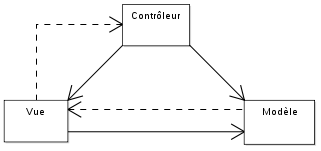
\includegraphics{ModeleMVC.png}
	\caption{Le modèle MVC}
	\label{modeleMVC}
	\end{figure}

	Lorsque l'utilisateur interagit avec les boutons de l'interface ou avec
	l'espace de jeu, celui-ci envoie une requête à l'application.
	Cette requête est envoyée depuis la vue puis analysée par le contrôleur.
	Ensuite, le contrôleur demande au modèle d'effectuer les traitements
	nécessaire. Enfin, le contrôleur renvoie la vue adaptée.

	\subsection{Les règles mises en place}
		\label{regles}

	Les différentes règles mises en place sont :
	
	\begin{itemize}
		\item Contrairement au Go le but premier est de faire une prise et la
		possesion de territoires~;
		\item Le suicide est interdit sauf s'il permet une prise~;
		\item Un pion ou un groupe de pions est pris lorsque celui-ci n'a plus de
		libertés~;
		\item Le jeu est fini lorsqu'un pion ou un groupe de pions est pris.
	\end{itemize}

	\subsection{Choix de l'algorithme d'I.A}
		\label{choix_alpha_beta}
	Pour ce jeu, nous avons choisi d'implémenter l'algorithme alpha-bêta. En
	effet, celui-ci est plus performant que l'algorithme min-max. Il donne les
	mêmes résultats au niveau de la stratégie mais est plus performant quant à la
	rapidité. Le gain produit par cette méthode est très important alors que les
	modifications à apporter à l'algorithme min-max sont simples.
	
\clearpage		
\section{Interface Homme-Machine}
L'IHM n'est pas le plus important de ce projet, cependant une IHM
représente quand même une partie importante du développement d'un projet.

Dans ce programme, l'IHM(Figure \ref{IHM_Vide}) est assez primaire avec une
barre de menu et le plateau de jeu :  le Goban.\\

	\begin{figure}[!ht]
    	\begin{center}
			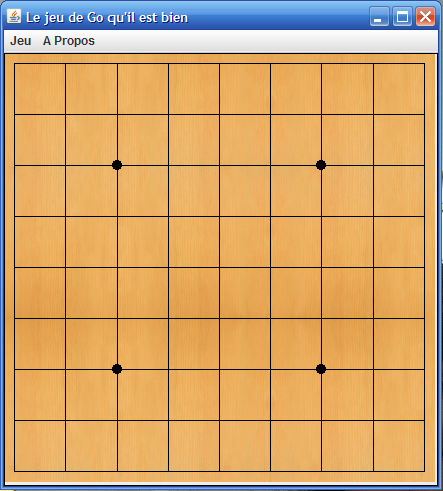
\includegraphics[scale=0.5]{IHM_Vide.png}
		\end{center}
	\caption{L'interface du programme}
	\label{IHM_Vide}
	\end{figure}

Cette IHM est constituée de deux parties :

	\begin{itemize}
  		\item Une partie correspondant au plateau de jeu~; 
		\item Une partie correspondant à la fenêtre de base(sans le Goban).\\
    \end{itemize}
    
Les menus sont constitués d'un sous-menu permettant le démarrage d'une nouvelle
partie et un autre qui sert à quitter l'application.\\

Toutes les interactions avec le Goban sont envoyés au modèle afin que les
différentes méthodes assurant le respect des règles de jeu, présentées dans la
section \ref{regles} soit lancées. Une fois ceci assuré, la vue est
actualisée afin que le pion apparraissent sur le plateau de jeu.
\clearpage
\section{Intelligence Artificielle}
L'intelligence artificielle est la partie la plus importante de ce projet car
c'est celle-ci qui constitue le lien entre ce programme et le module.
Pour réaliser cette intelligence, nous nous sommes basés sur l'algorithme
alpha-bêta vu en cours. Les raisons de ce choix ont été annoncés dans la
section \ref{choix_alpha_beta}.

\subsection{L'algorithme alpha-bêta}

\subsection{L'heuristique}
\clearpage
\section{Difficultés rencontrées}

\clearpage
\section{Conclusion}

\end{document}
